\section{Introdução}
\begin{frame}{Introdução}
	\begin{itemize}
	    \item Trabalho desenvolvido durante o intercâmbio internacional (BRAFITEC)
	    \item Tema do estágio profissional do último ano de curso da École nationale supérieure d'ingénieurs de Caen (ENSICAEN)
	    \item Estágio profissional sediado na Bootlin, empresa francesa especializada em Linux embarcado, localizada em Toulouse, França.
	\end{itemize}
\end{frame}

\begin{frame}{ENSICAEN}
\begin{itemize}
    \item École nationale supérieure d'ingénieurs de Caen
    \item Situada em Caen (França), na região da Normandia
    \item Dois anos de intercâmbio, na especialidade de Eletrônica e Física aplicada
\end{itemize}

\begin{figure}
    \centering
    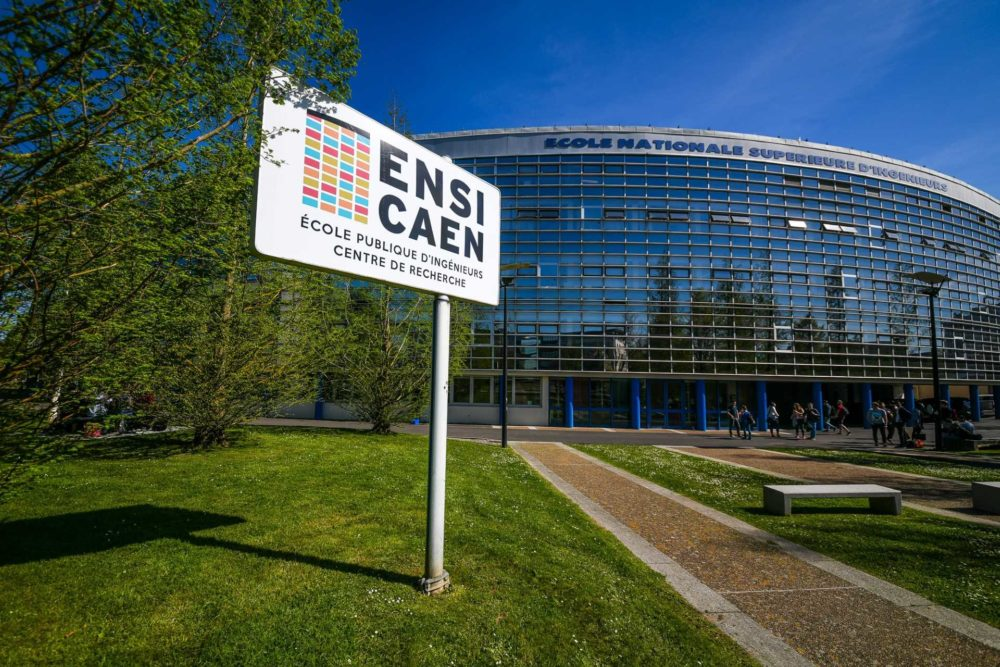
\includegraphics[width=0.4\columnwidth]{figuras/ENSICAEN-batiment-A.jpg}
    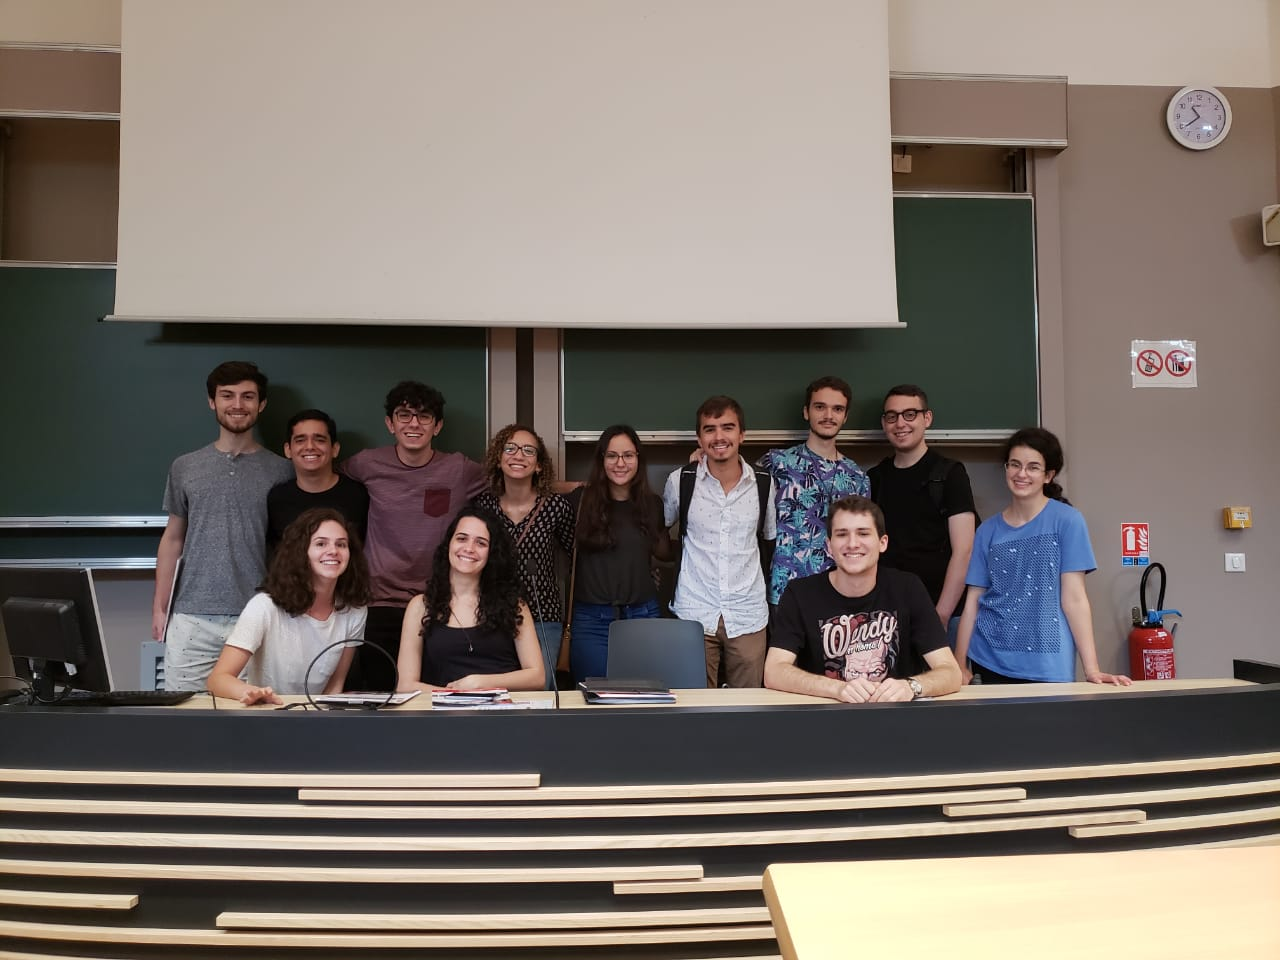
\includegraphics[scale=0.085]{figuras/pessoal_ensi.jpeg}
    %\caption{Caption}
    \label{fig:my_label}
\end{figure}
\end{frame}

\begin{frame}{Bootlin}
    \begin{itemize}
        \item Empresa prestadora de serviços e treinamentos em Linux embarcado
        \item Forte presença no mundo do software livre
        \item Escritórios em Toulouse, Lyon e Orange
    \end{itemize}
    
    \begin{figure}
        \centering
        
\includegraphics[scale=0.6]{figuras/bootlin_logo.png}
        %\caption{Logo da empresa}
        \label{fig:my_label}
    \end{figure}
\end{frame}


\begin{frame}{Contexto}
\begin{itemize}
    \item SquashFS é um sistema de arquivos comprimido e \textit{read-only}, amplamente utilizado
    \item Suportado pelo kernel Linux e por bootloaders populares como o Barebox
    \item U-Boot é o bootloader de código aberto mais popular para sistemas embarcados, mas não suportava o SquashFS até então
    \item Consequência: incapaz de ler partições formatadas com SquashFS
    \item Objetivo principal: adicionar o suporte ao SquashFS e integrá-lo ao código oficial do U-Boot
\end{itemize}
\end{frame}

\begin{frame}{Contexto}
\begin{center}
\begin{itemize}
    \item O suporte ao SquashFS é uma demanda antiga
    \item Requisitado pela comunidade do Linux embarcado
    \item Fluxo de trabalho: contribuir para um projeto de código aberto de destaque e entrar em contato com sua comunidade
\end{itemize}    

\begin{figure}
    \centering
    
\includegraphics[scale=0.06]{figuras/uboot_logo.png}
    %\caption{Caption}
    \label{fig:my_label}
\end{figure}
\end{center}
\end{frame}

\begin{frame}{SquashFS}
\begin{figure}
    \centering
    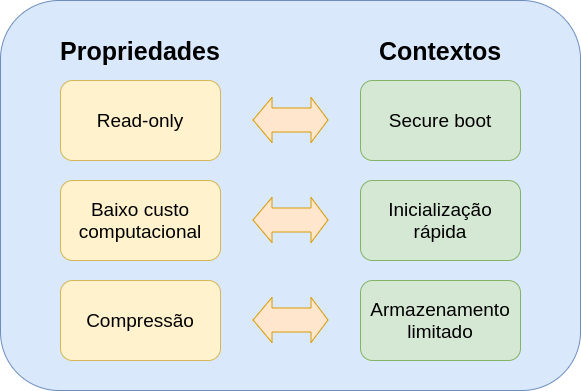
\includegraphics[scale=0.4]{figuras/squashfs_propriedades (1).png}
    %\caption{Caption}
    \label{fig:my_label}
\end{figure}
\end{frame}

\begin{frame}{Conceito-chave: bootloader}
    \begin{itemize}
        \item Carregar o kernel na memória RAM e inicializá-lo
        \item Soluções embarcadas populares: U-Boot e Barebox
        \item Soluções desktop: GRUB, Windows Boot Manager, etc.
    \end{itemize}
    
    \begin{figure}
        \centering
        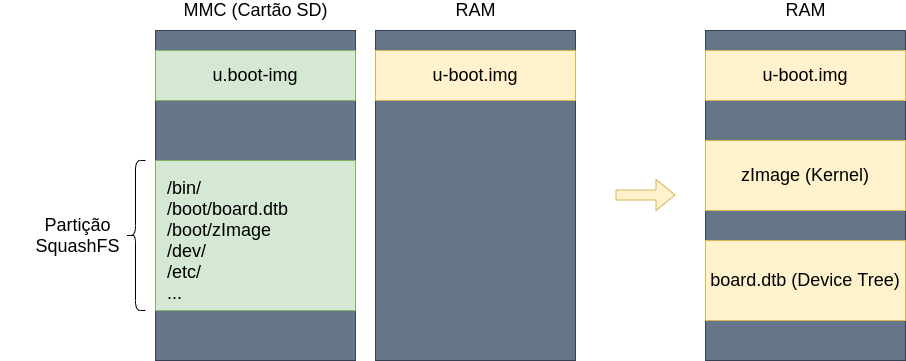
\includegraphics[scale=0.3]{figuras/bootloader.png}
        %\captionsetup{labelformat=empty}
        \caption{Funcionamento do bootloader}
        \label{fig:my_label}
    \end{figure}
\end{frame}

\begin{frame}{Conceito-chave: sistema de arquivos}
    
    \begin{itemize}
        \item Gerenciar o armazenamento de dados e metadados
        \item Oferece uma metodologia de organização para arquivos e pastas (diretórios)
        \item Implementado sob forma de arborescência
        \item Exemplos: SquashFS, FAT, ext*, NTFS, etc.
    \end{itemize}
    
\end{frame}

\begin{frame}{Conceito-chave: sistema de arquivos}
    \begin{columns}
    \begin{column}{0.5\textwidth}
    \begin{figure}
        \centering
        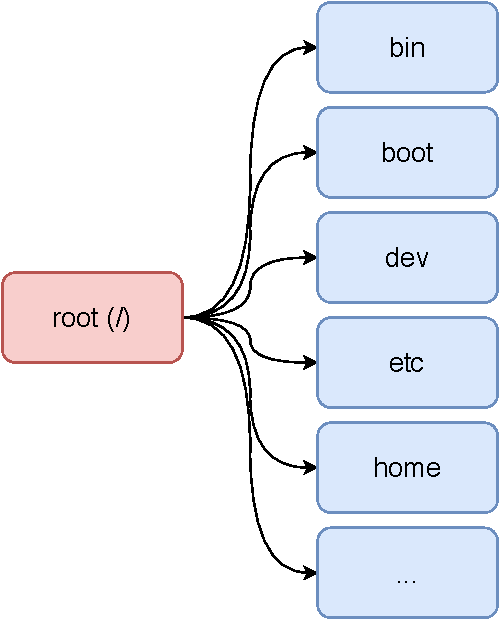
\includegraphics[scale=0.4]{figuras/FHS.pdf}
        \caption{Hierarquias de sistema de arquivo (padrão UNIX)}
        \label{fig:my_label}
    \end{figure}
    \end{column}
    \begin{column}{0.5\textwidth}
    \begin{figure}
        \centering
        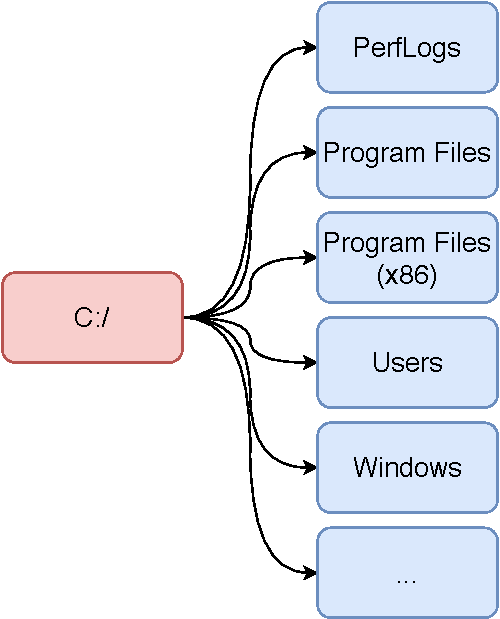
\includegraphics[scale=0.4]{figuras/windows.pdf}
        \caption{Hierarquias de sistema de arquivo no Windows}
        \label{fig:my_label}
    \end{figure}
    \end{column}
    
    \end{columns}
\end{frame}




 
